\section{HTTPS}

HTTPS is a protocol that extends the function of HTTP adding a layer of security, adapted to modern times. The bidirectional connection is encrypted using TLS (Transport Layer Security).
When TLS is used correctly, the connection between a user and a client has
\begin{itemize}
	\item \textbf{Privacy} Symmetric cryptography is used by both parties to transmit the data. The keys used are generated every session in a way that even if an eavesdropper has been supervising the  whole conversation cannot obtain said keys.
	\item \textbf{Authentication} The server can prove their identity using public key cryptography.
	\item \textbf{Integrity} The connection is considered reliable since every message contains an integrity check that ensures the data has not been modified
\end{itemize}
When connecting to a site that uses https, the URL begins with \textbf{https://} and the default port is \textbf{443} instead of 80


\subsubsection{TLS Handshake}
Before any data is transmitted, a TLS Handshake is performed. The goal of this handshake is to privately exchange the keys that will be used to encrypt the transmission and to authenticate the server. The protocol allows for the authentication of both the server and the client, but in this explanation we'll omit the client authentication as it is not used in usual HTTPS connections. 
\begin{enumerate}
\item The client sends a hello message that contains all the Cipher suites and versions supported, and a random number that will be used in the key exchange. If the client wants to resume a previous session, it only has to send the Session ID to resume it.

\item The server answers with the Cipher suite chosen (It should be the highest version available), the \textbf{sessionID}, another random number, and its digital certificate. The client then verifies that the certificate is signed by a trusted CA.

\item The client sends another random number encrypted with the server's public key (included in the digital certificate). This number is used to generate the symmetric key that will be used during the data exchange.

\item The client sends a finished message, that indicates that the handshake is completed

\item The server sends a finished message, that indicates that the handshake is completed

\item Data is exchanged and symmetrically encrypted. In this case, the data transmitted under TLS is plain HTTP.
\end{enumerate}

\begin{figure}[htb]
	\begin{centering}
		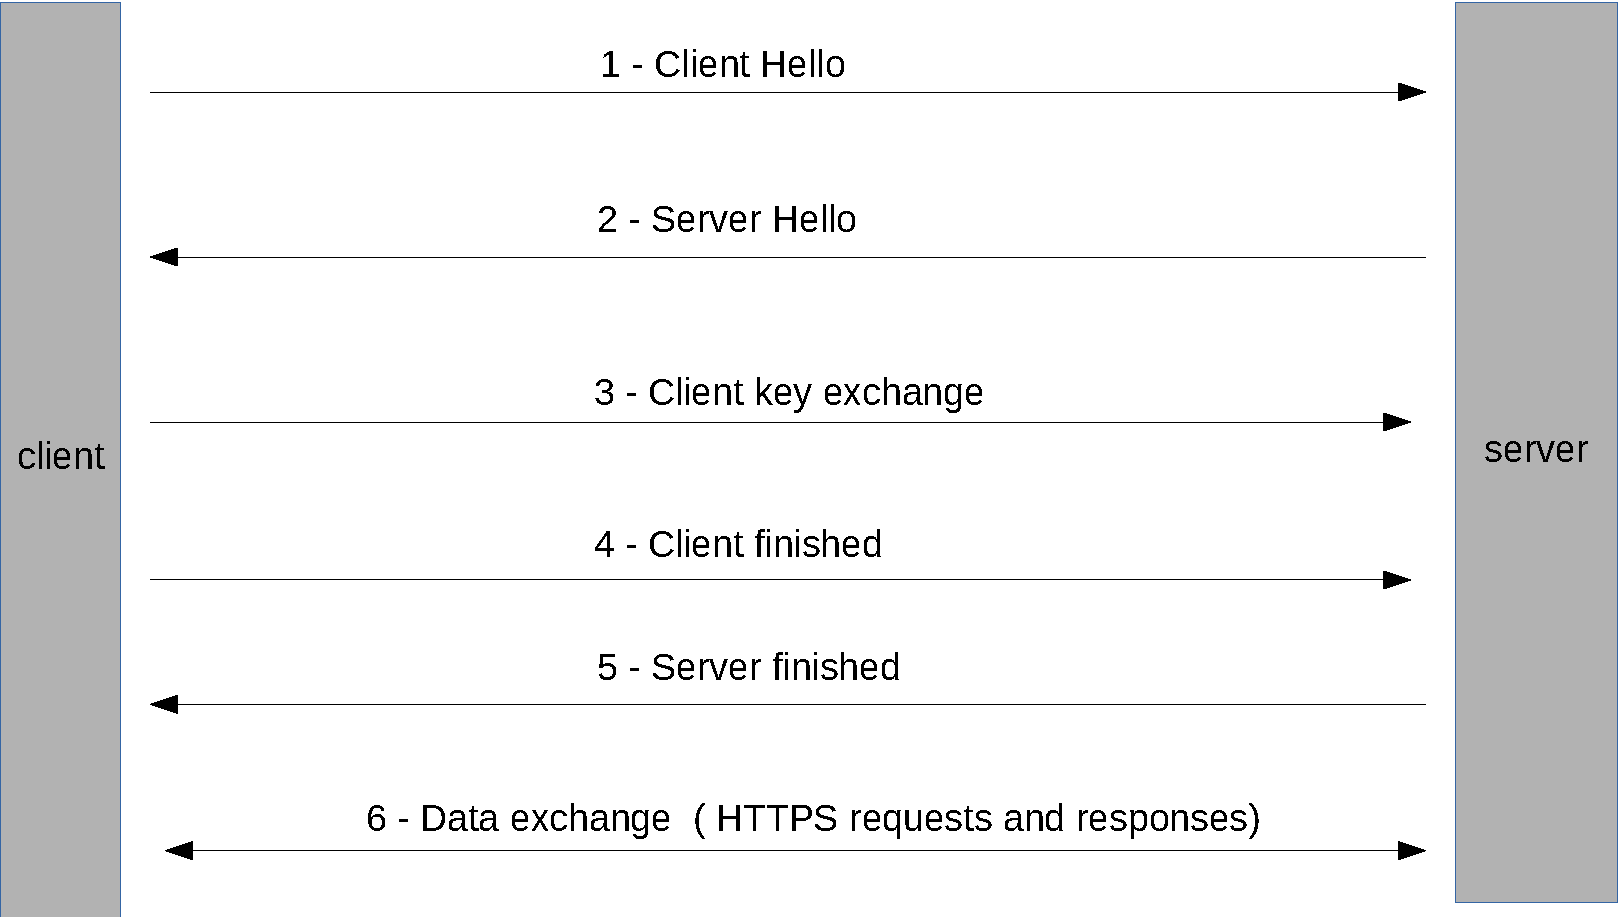
\includegraphics[width=0.7\columnwidth]{\securitydir/WebProtocols/figures/tls}
		\par
	\end{centering}
	\caption{\label{fig:tls} TLS handshake}
\end{figure}



\subsubsection{Public key certificates}
A public key certificate is an electronic document that the server uses to prove the ownership of a public key (therefore, its identity). Valid certificates have to be signed by a Certificate Authority (CA). A CA is a trusted third party (usually a company) that signs the certificates of the clients with its own certificate. Because it is not possible to have the certificates of all the CA that exist, their certificate is signed by another, called the \textbf{Root Certificate}. This root certificate is obtained when installing the operating system or the web browser. With this system we've established a \textbf{chain of trust}. When we visit a website we download its certificate. Then we check the CA that has issued it, and so on until we reach the root certificate. If the root certificate is found within the trusted by our system, we'll assume the certificate is valid, and that the server we are connecting to really owns this public key. 

\begin{figure}[htb]
	\begin{centering}
		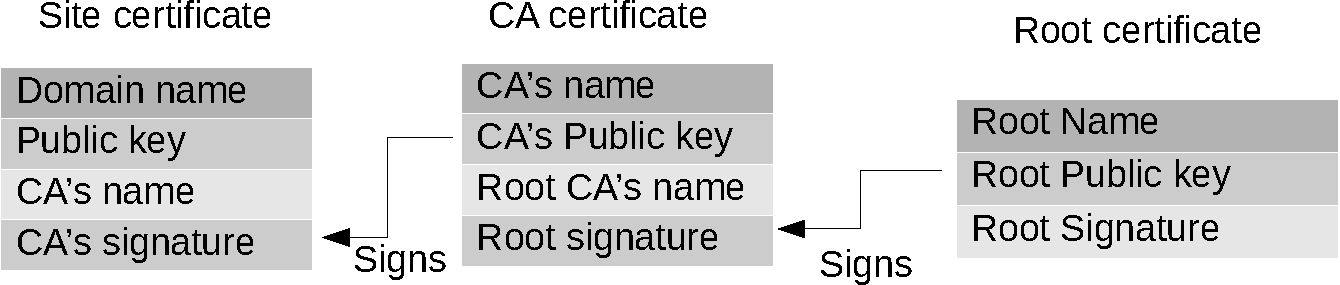
\includegraphics[width=0.7\columnwidth]{\securitydir/WebProtocols/figures/chain}
		\par
	\end{centering}
	\caption{\label{fig:chain} Chain of trust}
\end{figure}

A certificate contains the following information:
\begin{itemize}
	\item Owner's name (in a web context it would be the domain name)
	\item Owner's public key
	\item Name of the CA that has issued this certificate
	\item CA signature of the certificate.
	\item Valid time.
\end{itemize}


\subsection{HTTP Strict Transport Security (HSTS)} 
HSTS is a mechanism used by the web servers to tell browsers that they should only interact with them using HTTPS. When HTSTS is enabled on a server, the server responds the requests with the header \textbf{Strict-Transport-Security} indicating a time period in seconds on which the browser should only use HTTPS to connect to that domain. Browsers should do the following when contacting a HSTS enabled domain.
\begin{itemize}
	\item Always connect via https. If the user introduces a link that begins with http://, automatically transform it to https. The browser should never attempt to do any connection via http.
	\item If the certificate is not valid (expired, self signed, etc), the browser should terminate the connection immediately.
\end{itemize}

To enable HSTS on a website, the server should respond to any request with the following header specifying a TTL in seconds.
\begin{lstlisting}[style=verbs]
Strict-Transport-Security: max-age=31536000
\end{lstlisting}
When a browser gets this header, it automatically applies the standard for this site during the specified time.

\paragraph{Preloaded HSTS}
HSTS can also be \textbf{preloaded.} This means that browser are installed with a default list of domains that have requested to be included in it. If a domain is in this list, the browser will apply HSTS by default, without waiting to receive any header. This is done because even though HSTS greatly improves security, the first connection is still vulnerable.

\paragraph{Downgrade attacks}
The mechanism is used to protect the connection from \textbf{downgrade attacks}. If a malicious agent could poison the dns responses for a user in order to point them to a server that he controls, he could be able to use a proxy that establishes a http connection to the user and a https connection to the original server. The user would only see that the connection is https, but for most users that would not raise any suspicion.

\begin{figure}[htb]
	\begin{centering}
		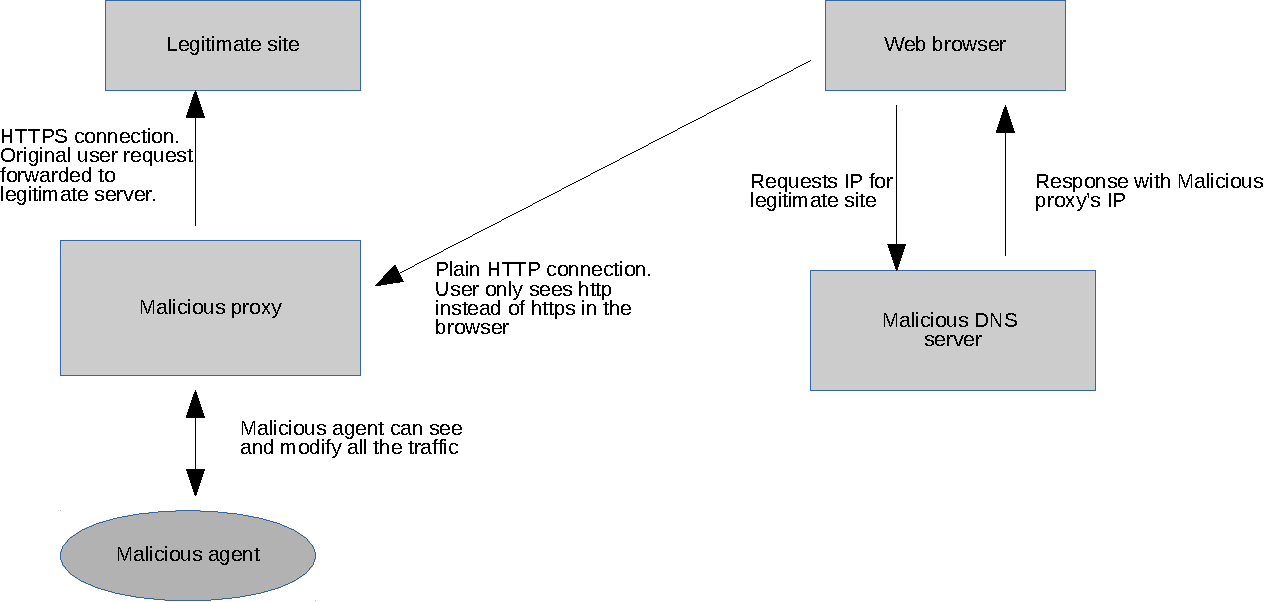
\includegraphics[width=0.7\columnwidth]{\securitydir/WebProtocols/figures/hsts}
		\par
	\end{centering}
	\caption{\label{fig:hsts} Downgrade attack without HSTS enabled}
\end{figure}

If HSTS was enabled in this scenario, the browser would refuse to connect to the proxy as the connection was plain http. 


\paragraph{Server Name Indication (SNI)}
Since IP addresses are scarce, it is not unusual to host several websites under the same IP. If we are working with HTTP in this IP we have usually have a reverse proxy, that reads the \textbf{Host} field of the request that indicates the domain of the website we are connecting to, and forwards the request to the correct web server. This works well in HTTP, but what about HTTPS?. In HTTPS when the client initiates a TLS connection, the server does not know which server the client is connecting to, and therefore the server does not know which digital certificate send (assuming the different sites have different digital certificates). If the server sends the wrong certificate, the client browser won't trust the server, as the certificate won't match the request.

SNI fixes this problem by sending the domain name as part of the TLS negotiation. This way, the server knows which certificate send and the the TLS handshake works as usual. It is important to known that the domain name is sent unencrypted, so third parties can know which domain the client is connecting to.

\paragraph{Mixed content}
%TODO ...